\SourceLeaf{263}%
\begin{center}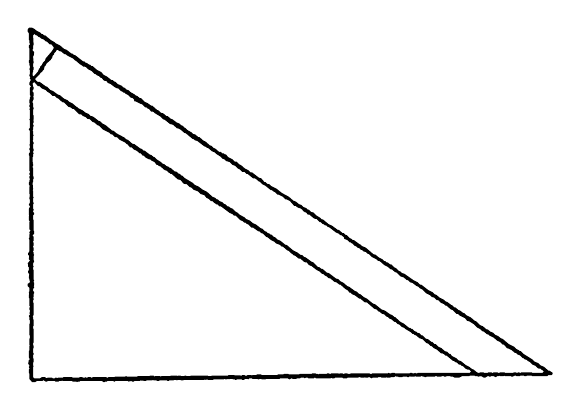
\begin{tikzpicture}[x=0.00688299cm,y=-0.00688299cm]
\fill[even odd rule] (25,22) -- (24,24) -- (24,27) -- (26,30) -- (26,42) -- (27,43) -- (27,48) -- (28,49) -- (28,51) -- (26,53) -- (26,57) -- (27,58) -- (27,80) -- (26,81) -- (26,84) -- (27,85) -- (27,89) -- (28,90) -- (28,95) -- (27,96) -- (28,98) -- (28,106) -- (27,107) -- (27,109) -- (29,111) -- (28,114) -- (30,116) -- (27,122) -- (27,125) -- (30,128) -- (30,129) -- (28,131) -- (28,144) -- (29,145) -- (29,148) -- (28,149) -- (28,152) -- (27,153) -- (27,159) -- (28,160) -- (28,162) -- (27,163) -- (27,166) -- (28,167) -- (28,169) -- (27,170) -- (28,172) -- (28,188) -- (27,189) -- (28,191) -- (28,205) -- (26,207) -- (26,208) -- (28,210) -- (28,235) -- (27,236) -- (28,238) -- (28,242) -- (27,243) -- (27,245) -- (28,246) -- (28,250) -- (26,253) -- (26,255) -- (27,256) -- (27,284) -- (28,285) -- (28,288) -- (27,289) -- (27,291) -- (28,292) -- (28,294) -- (27,295) -- (28,301) -- (27,302) -- (27,305) -- (26,306) -- (26,309) -- (28,312) -- (27,314) -- (27,327) -- (28,328) -- (27,336) -- (28,337) -- (28,343) -- (26,347) -- (28,349) -- (28,351) -- (26,355) -- (26,365) -- (27,366) -- (26,368) -- (26,375) -- (28,377) -- (27,379) -- (27,392) -- (29,394) -- (29,395) -- (27,397) -- (27,399) -- (28,400) -- (27,402) -- (27,408) -- (26,409) -- (27,411) -- (27,433) -- (25,436) -- (25,439) -- (27,441) -- (26,447) -- (28,449) -- (28,450) -- (24,455) -- (25,457) -- (25,461) -- (26,462) -- (26,468) -- (25,469) -- (25,472) -- (27,475) -- (26,482) -- (27,483) -- (27,486) -- (28,487) -- (28,490) -- (24,493) -- (24,497) -- (27,500) -- (27,507) -- (26,508) -- (27,512) -- (26,513) -- (26,518) -- (27,519) -- (27,533) -- (28,534) -- (28,536) -- (27,537) -- (27,540) -- (28,541) -- (28,545) -- (27,547) -- (28,548) -- (28,550) -- (26,552) -- (27,554) -- (27,559) -- (28,560) -- (28,566) -- (27,567) -- (27,587) -- (28,588) -- (28,593) -- (27,594) -- (27,605) -- (28,607) -- (27,608) -- (27,616) -- (26,617) -- (26,628) -- (28,632) -- (26,634) -- (25,640) -- (27,643) -- (27,645) -- (26,646) -- (27,648) -- (27,650) -- (26,651) -- (26,657) -- (27,658) -- (27,668) -- (32,674) -- (38,674) -- (41,672) -- (51,672) -- (52,671) -- (54,671) -- (57,673) -- (60,673) -- (61,672) -- (74,672) -- (75,673) -- (81,673) -- (82,672) -- (86,672) -- (88,671) -- (89,672) -- (106,672) -- (107,673) -- (114,673) -- (115,674) -- (117,673) -- (120,673) -- (121,672) -- (161,672) -- (164,674) -- (166,674) -- (167,673) -- (170,673) -- (171,672) -- (182,672) -- (183,673) -- (185,673) -- (186,672) -- (209,672) -- (210,673) -- (216,672) -- (217,673) -- (220,673) -- (221,672) -- (231,672) -- (232,671) -- (242,672) -- (243,671) -- (254,671) -- (255,670) -- (257,671) -- (262,671) -- (263,672) -- (266,672) -- (267,671) -- (281,671) -- (282,672) -- (284,672) -- (285,671) -- (293,671) -- (294,670) -- (298,670) -- (299,671) -- (301,670) -- (306,670) -- (307,671) -- (311,671) -- (312,670) -- (350,670) -- (351,669) -- (353,670) -- (355,669) -- (357,670) -- (366,670) -- (367,669) -- (386,669) -- (387,668) -- (389,669) -- (402,668) -- (403,669) -- (406,669) -- (407,670) -- (409,670) -- (410,669) -- (419,669) -- (420,670) -- (423,670) -- (425,668) -- (429,668) -- (431,669) -- (433,667) -- (438,667) -- (439,668) -- (448,668) -- (449,669) -- (451,669) -- (452,668) -- (455,668) -- (456,669) -- (463,669) -- (464,668) -- (489,668) -- (490,667) -- (504,667) -- (507,669) -- (511,667) -- (513,668) -- (520,668) -- (521,667) -- (527,667) -- (528,666) -- (534,666) -- (535,667) -- (537,666) -- (541,666) -- (542,667) -- (552,667) -- (553,666) -- (555,666) -- (556,667) -- (583,667) -- (584,666) -- (586,667) -- (590,667) -- (591,666) -- (605,666) -- (606,667) -- (613,667) -- (614,666) -- (634,666) -- (635,665) -- (638,665) -- (639,666) -- (645,666) -- (646,665) -- (648,666) -- (652,666) -- (653,665) -- (655,665) -- (659,667) -- (660,666) -- (670,666) -- (671,665) -- (676,665) -- (677,666) -- (685,666) -- (686,665) -- (688,666) -- (693,666) -- (694,665) -- (700,665) -- (703,663) -- (705,664) -- (708,664) -- (709,665) -- (715,665) -- (716,664) -- (724,664) -- (725,665) -- (727,665) -- (729,663) -- (731,664) -- (738,664) -- (739,663) -- (741,664) -- (749,664) -- (750,663) -- (752,663) -- (753,664) -- (756,664) -- (757,665) -- (759,665) -- (760,664) -- (775,664) -- (776,663) -- (779,663) -- (780,664) -- (787,664) -- (788,663) -- (792,663) -- (793,664) -- (796,664) -- (797,663) -- (804,663) -- (805,664) -- (809,664) -- (812,666) -- (820,666) -- (826,663) -- (839,663) -- (840,662) -- (849,662) -- (850,663) -- (854,663) -- (855,664) -- (861,663) -- (866,666) -- (868,666) -- (873,663) -- (875,663) -- (876,664) -- (878,664) -- (879,663) -- (884,663) -- (888,665) -- (890,663) -- (893,663) -- (894,662) -- (896,663) -- (902,663) -- (903,662) -- (905,663) -- (916,663) -- (917,664) -- (919,664) -- (923,662) -- (925,662) -- (926,663) -- (932,663) -- (933,662) -- (940,662) -- (941,663) -- (944,663) -- (945,662) -- (954,662) -- (955,663) -- (983,663) -- (985,661) -- (991,661) -- (993,659) -- (993,657) -- (987,653) -- (985,653) -- (977,646) -- (970,643) -- (966,639) -- (959,636) -- (955,632) -- (939,622) -- (934,617) -- (932,617) -- (930,615) -- (926,613) -- (922,609) -- (912,604) -- (900,594) -- (897,593) -- (892,589) -- (887,587) -- (883,583) -- (878,581) -- (873,577) -- (871,577) -- (864,571) -- (859,569) -- (852,562) -- (849,561) -- (842,555) -- (834,551) -- (830,547) -- (827,546) -- (822,542) -- (819,541) -- (813,536) -- (811,536) -- (807,532) -- (806,532) -- (798,526) -- (795,525) -- (792,522) -- (784,518) -- (778,513) -- (775,512) -- (771,508) -- (763,504) -- (750,494) -- (748,494) -- (744,490) -- (736,486) -- (719,474) -- (715,473) -- (712,470) -- (709,469) -- (704,464) -- (700,462) -- (695,457) -- (693,457) -- (688,453) -- (686,453) -- (684,451) -- (682,451) -- (678,447) -- (672,444) -- (666,439) -- (662,438) -- (648,426) -- (641,423) -- (638,420) -- (637,420) -- (626,412) -- (624,412) -- (622,410) -- (618,408) -- (613,403) -- (610,402) -- (607,399) -- (605,399) -- (598,393) -- (596,393) -- (585,385) -- (580,383) -- (569,374) -- (567,374) -- (564,371) -- (556,366) -- (551,361) -- (547,360) -- (543,356) -- (541,356) -- (538,353) -- (533,351) -- (529,347) -- (525,346) -- (519,341) -- (514,339) -- (506,332) -- (493,325) -- (483,317) -- (473,312) -- (470,309) -- (466,308) -- (463,305) -- (461,305) -- (455,298) -- (451,297) -- (438,287) -- (435,287) -- (431,283) -- (425,280) -- (418,274) -- (414,272) -- (409,267) -- (406,267) -- (402,263) -- (394,259) -- (390,254) -- (388,254) -- (386,252) -- (383,252) -- (380,249) -- (377,249) -- (370,243) -- (367,242) -- (363,238) -- (360,237) -- (352,230) -- (349,229) -- (341,222) -- (339,222) -- (333,217) -- (329,216) -- (326,213) -- (319,209) -- (315,205) -- (314,205) -- (310,201) -- (307,200) -- (304,197) -- (299,195) -- (291,189) -- (288,188) -- (282,183) -- (280,183) -- (274,178) -- (270,177) -- (266,173) -- (263,172) -- (254,164) -- (252,164) -- (245,159) -- (240,157) -- (233,150) -- (231,150) -- (226,146) -- (223,145) -- (221,143) -- (214,139) -- (211,136) -- (206,134) -- (203,131) -- (200,130) -- (197,127) -- (190,124) -- (186,120) -- (183,119) -- (181,117) -- (179,117) -- (170,110) -- (164,107) -- (160,102) -- (152,98) -- (144,91) -- (142,91) -- (139,88) -- (137,88) -- (133,85) -- (131,85) -- (128,82) -- (126,82) -- (112,71) -- (109,70) -- (107,68) -- (105,68) -- (96,61) -- (91,59) -- (84,53) -- (76,49) -- (74,47) -- (67,43) -- (56,34) -- (54,34) -- (52,32) -- (50,32) -- (47,29) -- (41,26) -- (36,22) -- (32,20) -- (27,20) -- cycle
(33,123) -- (35,121) -- (37,121) -- (43,128) -- (46,128) -- (50,132) -- (57,135) -- (60,138) -- (65,141) -- (70,146) -- (74,146) -- (77,149) -- (81,151) -- (86,156) -- (87,156) -- (89,158) -- (91,158) -- (99,166) -- (103,167) -- (107,170) -- (109,170) -- (118,179) -- (120,180) -- (123,180) -- (126,183) -- (131,185) -- (134,188) -- (139,189) -- (144,194) -- (147,195) -- (153,200) -- (156,201) -- (163,208) -- (175,214) -- (178,217) -- (180,217) -- (185,222) -- (188,222) -- (190,223) -- (194,227) -- (204,232) -- (207,235) -- (208,235) -- (213,241) -- (216,241) -- (220,245) -- (225,247) -- (231,252) -- (233,252) -- (236,256) -- (238,256) -- (242,260) -- (248,263) -- (250,263) -- (252,265) -- (258,268) -- (262,273) -- (264,273) -- (266,275) -- (269,276) -- (277,283) -- (281,284) -- (285,288) -- (286,288) -- (288,290) -- (290,290) -- (301,300) -- (306,301) -- (312,308) -- (318,309) -- (323,314) -- (326,315) -- (330,319) -- (338,322) -- (343,327) -- (350,329) -- (354,334) -- (358,336) -- (362,340) -- (365,340) -- (369,344) -- (370,344) -- (372,346) -- (374,346) -- (378,350) -- (381,350) -- (397,362) -- (402,364) -- (405,367) -- (408,367) -- (416,375) -- (421,377) -- (424,380) -- (426,380) -- (428,382) -- (431,383) -- (437,389) -- (440,389) -- (450,396) -- (452,396) -- (455,399) -- (458,400) -- (464,406) -- (467,407) -- (473,412) -- (479,415) -- (482,418) -- (490,421) -- (493,424) -- (495,424) -- (503,431) -- (506,432) -- (511,437) -- (512,437) -- (515,440) -- (518,441) -- (524,446) -- (527,446) -- (534,452) -- (536,453) -- (539,453) -- (543,458) -- (548,460) -- (557,467) -- (563,470) -- (567,474) -- (570,475) -- (572,477) -- (576,479) -- (579,482) -- (583,483) -- (590,489) -- (594,490) -- (599,494) -- (601,494) -- (610,502) -- (615,505) -- (618,509) -- (620,509) -- (623,512) -- (628,514) -- (636,520) -- (638,520) -- (645,526) -- (647,527) -- (650,527) -- (664,539) -- (668,540) -- (672,544) -- (673,544) -- (678,548) -- (682,549) -- (686,553) -- (689,554) -- (692,557) -- (695,558) -- (701,563) -- (703,563) -- (707,567) -- (710,568) -- (714,572) -- (719,574) -- (721,576) -- (731,582) -- (734,585) -- (736,585) -- (738,587) -- (741,588) -- (747,593) -- (753,595) -- (760,602) -- (763,603) -- (767,607) -- (770,608) -- (773,611) -- (779,614) -- (787,621) -- (789,621) -- (793,623) -- (795,625) -- (797,625) -- (809,635) -- (811,635) -- (813,637) -- (816,638) -- (820,642) -- (823,642) -- (825,644) -- (828,645) -- (832,649) -- (836,651) -- (839,651) -- (842,654) -- (842,655) -- (840,657) -- (744,657) -- (743,658) -- (740,658) -- (739,657) -- (737,658) -- (734,658) -- (733,657) -- (730,657) -- (729,658) -- (702,658) -- (701,657) -- (696,657) -- (695,658) -- (692,658) -- (690,657) -- (689,658) -- (660,658) -- (659,659) -- (656,659) -- (655,658) -- (620,658) -- (619,659) -- (615,659) -- (614,658) -- (609,658) -- (608,659) -- (606,659) -- (605,658) -- (600,658) -- (599,659) -- (597,658) -- (584,658) -- (583,659) -- (581,659) -- (580,658) -- (577,658) -- (576,659) -- (562,659) -- (561,660) -- (559,659) -- (556,659) -- (555,658) -- (549,658) -- (548,659) -- (526,659) -- (525,660) -- (506,660) -- (505,659) -- (497,659) -- (496,660) -- (486,660) -- (485,661) -- (456,661) -- (455,660) -- (447,660) -- (446,661) -- (439,661) -- (438,662) -- (436,661) -- (430,661) -- (429,662) -- (425,662) -- (424,661) -- (420,661) -- (419,662) -- (395,661) -- (394,662) -- (364,662) -- (363,663) -- (357,663) -- (356,662) -- (325,662) -- (324,663) -- (317,663) -- (316,662) -- (314,662) -- (313,663) -- (307,663) -- (306,662) -- (302,662) -- (301,663) -- (299,662) -- (288,662) -- (287,663) -- (271,663) -- (270,664) -- (268,663) -- (260,663) -- (258,664) -- (256,662) -- (250,662) -- (249,663) -- (227,663) -- (226,664) -- (207,664) -- (206,663) -- (204,664) -- (185,664) -- (184,665) -- (173,665) -- (172,666) -- (170,666) -- (169,665) -- (144,665) -- (143,666) -- (141,666) -- (140,665) -- (135,665) -- (134,666) -- (132,666) -- (131,665) -- (129,666) -- (126,666) -- (125,665) -- (120,665) -- (119,666) -- (107,666) -- (106,665) -- (90,665) -- (89,666) -- (80,666) -- (79,667) -- (77,666) -- (75,666) -- (74,667) -- (70,667) -- (69,666) -- (61,666) -- (59,667) -- (56,665) -- (50,665) -- (47,667) -- (36,667) -- (34,665) -- (34,646) -- (35,645) -- (34,643) -- (34,638) -- (35,637) -- (35,631) -- (34,630) -- (34,624) -- (35,623) -- (35,621) -- (34,620) -- (34,612) -- (35,611) -- (35,607) -- (34,606) -- (34,602) -- (35,601) -- (35,576) -- (34,575) -- (34,571) -- (35,570) -- (35,559) -- (34,558) -- (34,554) -- (33,553) -- (35,550) -- (35,528) -- (34,527) -- (34,523) -- (35,522) -- (35,520) -- (34,518) -- (35,517) -- (35,511) -- (36,510) -- (36,508) -- (34,506) -- (34,502) -- (36,500) -- (36,498) -- (35,497) -- (36,495) -- (36,491) -- (35,490) -- (35,488) -- (36,487) -- (35,485) -- (35,467) -- (34,466) -- (34,462) -- (35,461) -- (34,459) -- (34,455) -- (36,451) -- (35,449) -- (35,441) -- (36,439) -- (35,438) -- (35,435) -- (34,434) -- (34,432) -- (35,431) -- (35,426) -- (34,425) -- (34,423) -- (35,422) -- (35,417) -- (34,416) -- (34,414) -- (35,413) -- (35,406) -- (33,404) -- (33,403) -- (36,400) -- (36,396) -- (35,395) -- (35,375) -- (34,374) -- (34,366) -- (36,364) -- (36,362) -- (34,360) -- (34,358) -- (35,357) -- (35,355) -- (34,354) -- (34,346) -- (35,345) -- (35,343) -- (34,342) -- (34,335) -- (35,333) -- (34,332) -- (34,321) -- (33,320) -- (34,318) -- (33,306) -- (34,305) -- (34,300) -- (35,299) -- (35,295) -- (34,294) -- (34,279) -- (33,278) -- (33,276) -- (34,275) -- (34,271) -- (33,270) -- (34,269) -- (33,268) -- (33,259) -- (34,258) -- (34,253) -- (35,252) -- (34,250) -- (34,248) -- (35,247) -- (35,244) -- (34,243) -- (34,235) -- (35,234) -- (35,232) -- (33,229) -- (34,227) -- (34,220) -- (35,219) -- (34,217) -- (34,211) -- (33,210) -- (34,208) -- (34,203) -- (35,202) -- (35,200) -- (34,199) -- (34,196) -- (35,195) -- (35,192) -- (34,191) -- (35,189) -- (35,182) -- (34,181) -- (34,171) -- (35,170) -- (35,168) -- (34,167) -- (34,160) -- (33,159) -- (33,156) -- (35,152) -- (35,149) -- (34,148) -- (35,146) -- (35,140) -- (33,138) -- (33,136) -- (35,133) -- (35,130) -- (34,129) -- cycle
(38,114) -- (47,105) -- (47,104) -- (51,101) -- (51,100) -- (54,97) -- (55,92) -- (57,90) -- (59,86) -- (67,79) -- (67,78) -- (69,76) -- (70,72) -- (73,69) -- (73,67) -- (76,64) -- (76,63) -- (78,61) -- (80,61) -- (82,63) -- (86,64) -- (92,69) -- (94,69) -- (98,72) -- (108,77) -- (112,81) -- (113,81) -- (121,88) -- (122,88) -- (127,92) -- (130,92) -- (132,93) -- (136,97) -- (142,100) -- (147,105) -- (150,106) -- (152,108) -- (155,109) -- (158,112) -- (161,113) -- (164,117) -- (166,118) -- (169,118) -- (172,122) -- (177,124) -- (185,130) -- (189,132) -- (191,132) -- (196,137) -- (199,138) -- (201,140) -- (203,140) -- (205,142) -- (209,144) -- (214,149) -- (218,150) -- (220,152) -- (221,156) -- (223,156) -- (233,161) -- (235,161) -- (241,167) -- (243,167) -- (245,169) -- (248,170) -- (252,175) -- (255,175) -- (257,176) -- (259,178) -- (269,184) -- (274,189) -- (277,190) -- (287,198) -- (292,199) -- (300,206) -- (302,206) -- (306,208) -- (313,214) -- (316,215) -- (328,225) -- (331,226) -- (333,228) -- (337,229) -- (350,239) -- (353,240) -- (355,242) -- (357,242) -- (364,248) -- (369,250) -- (372,253) -- (380,258) -- (384,262) -- (387,263) -- (390,266) -- (397,268) -- (402,273) -- (407,275) -- (412,280) -- (416,282) -- (420,286) -- (424,286) -- (428,290) -- (430,290) -- (440,298) -- (443,298) -- (445,299) -- (451,304) -- (452,304) -- (457,309) -- (463,312) -- (473,320) -- (475,320) -- (477,322) -- (481,324) -- (485,328) -- (487,328) -- (495,332) -- (500,337) -- (502,337) -- (508,340) -- (516,349) -- (519,349) -- (521,351) -- (525,353) -- (527,353) -- (529,355) -- (530,355) -- (533,359) -- (534,359) -- (536,361) -- (538,361) -- (541,365) -- (544,365) -- (551,371) -- (555,373) -- (557,373) -- (563,379) -- (565,379) -- (568,382) -- (571,383) -- (573,385) -- (575,385) -- (578,388) -- (580,388) -- (593,398) -- (598,400) -- (601,403) -- (603,403) -- (608,407) -- (608,409) -- (609,410) -- (614,412) -- (618,416) -- (620,416) -- (622,418) -- (623,418) -- (628,423) -- (630,423) -- (633,426) -- (636,427) -- (639,430) -- (641,430) -- (644,433) -- (648,434) -- (651,437) -- (654,438) -- (659,443) -- (667,447) -- (670,450) -- (674,451) -- (682,458) -- (688,461) -- (694,466) -- (696,466) -- (702,471) -- (705,472) -- (712,479) -- (718,481) -- (724,486) -- (726,486) -- (730,490) -- (734,491) -- (742,497) -- (745,498) -- (748,501) -- (752,503) -- (759,510) -- (767,514) -- (770,517) -- (774,518) -- (779,523) -- (782,523) -- (787,528) -- (792,530) -- (795,533) -- (797,533) -- (805,540) -- (808,541) -- (815,548) -- (818,548) -- (821,551) -- (831,556) -- (835,561) -- (839,562) -- (847,567) -- (853,573) -- (859,576) -- (863,580) -- (866,581) -- (872,586) -- (874,586) -- (876,588) -- (884,592) -- (891,598) -- (896,600) -- (901,605) -- (903,605) -- (909,612) -- (911,612) -- (917,615) -- (923,620) -- (925,620) -- (928,623) -- (933,625) -- (938,630) -- (939,630) -- (941,632) -- (945,633) -- (947,635) -- (951,637) -- (956,642) -- (961,644) -- (965,648) -- (967,649) -- (970,649) -- (973,652) -- (974,652) -- (976,654) -- (976,655) -- (974,657) -- (955,657) -- (954,656) -- (935,656) -- (934,657) -- (932,657) -- (931,656) -- (929,656) -- (928,657) -- (926,657) -- (925,656) -- (921,656) -- (920,657) -- (905,657) -- (904,656) -- (896,656) -- (895,657) -- (892,657) -- (891,656) -- (884,656) -- (883,657) -- (881,657) -- (880,656) -- (874,656) -- (873,657) -- (866,657) -- (865,656) -- (859,656) -- (858,657) -- (855,657) -- (853,656) -- (847,651) -- (844,650) -- (839,646) -- (833,643) -- (823,635) -- (819,634) -- (815,630) -- (807,626) -- (804,622) -- (802,622) -- (798,618) -- (794,617) -- (787,611) -- (782,609) -- (777,604) -- (775,604) -- (771,600) -- (769,600) -- (763,595) -- (759,594) -- (753,588) -- (751,588) -- (747,584) -- (743,583) -- (741,581) -- (738,580) -- (734,576) -- (732,576) -- (730,574) -- (728,574) -- (718,566) -- (712,563) -- (702,554) -- (701,554) -- (696,550) -- (693,549) -- (683,542) -- (677,540) -- (666,531) -- (661,529) -- (650,520) -- (644,517) -- (638,512) -- (635,511) -- (631,507) -- (628,506) -- (617,498) -- (614,497) -- (607,491) -- (601,488) -- (597,484) -- (593,483) -- (580,473) -- (576,472) -- (568,465) -- (566,465) -- (562,462) -- (560,462) -- (551,453) -- (548,452) -- (537,444) -- (534,443) -- (531,440) -- (527,439) -- (522,435) -- (514,431) -- (502,421) -- (500,421) -- (490,413) -- (485,411) -- (481,407) -- (478,406) -- (474,402) -- (472,402) -- (470,400) -- (467,399) -- (464,396) -- (462,396) -- (457,391) -- (454,390) -- (445,383) -- (440,381) -- (434,376) -- (427,373) -- (424,370) -- (415,365) -- (412,362) -- (407,359) -- (402,354) -- (399,353) -- (395,350) -- (393,350) -- (389,346) -- (386,345) -- (383,342) -- (378,340) -- (375,337) -- (373,337) -- (370,334) -- (365,332) -- (355,323) -- (347,319) -- (339,313) -- (332,310) -- (328,306) -- (313,297) -- (309,293) -- (308,293) -- (305,290) -- (302,289) -- (299,286) -- (295,285) -- (288,279) -- (285,278) -- (283,276) -- (281,276) -- (276,272) -- (273,271) -- (270,268) -- (262,263) -- (258,259) -- (257,259) -- (252,255) -- (249,254) -- (240,247) -- (238,247) -- (235,244) -- (232,243) -- (221,235) -- (217,234) -- (209,227) -- (206,226) -- (203,223) -- (188,215) -- (182,210) -- (180,210) -- (168,200) -- (162,197) -- (158,193) -- (155,192) -- (146,185) -- (142,183) -- (140,183) -- (136,179) -- (131,177) -- (126,173) -- (118,169) -- (115,166) -- (114,166) -- (107,160) -- (101,157) -- (98,154) -- (91,151) -- (84,145) -- (79,143) -- (71,137) -- (66,135) -- (60,129) -- (57,128) -- (46,120) -- (43,120) -- (41,119) -- (38,116) -- cycle
(37,32) -- (39,34) -- (41,34) -- (44,37) -- (47,38) -- (49,40) -- (54,42) -- (57,45) -- (60,46) -- (65,51) -- (68,51) -- (72,56) -- (72,58) -- (69,63) -- (57,77) -- (56,81) -- (52,85) -- (50,89) -- (47,92) -- (47,94) -- (45,96) -- (43,101) -- (35,110) -- (33,108) -- (33,103) -- (34,102) -- (34,98) -- (35,97) -- (35,93) -- (34,92) -- (34,86) -- (35,85) -- (34,73) -- (35,72) -- (36,65) -- (33,62) -- (33,60) -- (34,59) -- (34,53) -- (35,52) -- (34,34) -- (36,32) -- cycle;
\end{tikzpicture}
\end{center}

\noindent Ferner folgt durch Construction dass f\"ur $A = \text{const.}$:

\[
\sin B\,.\,\partial a = gc\,.\,\sin A\,.\,\partial b,
\]

\noindent also durch Verbindung von III. und 2)

\[
ga\,.\,\cos B = gc\,.\,\sin A
\]

\noindent und

\[
\tag*{3)} ga\,.\,gb = gc
\]

\[
\tag*{4)} \operatorname{tg}A\operatorname{tg}B\,.\,gc = 1.
\]

\Needspace{23\baselineskip}
\begin{center}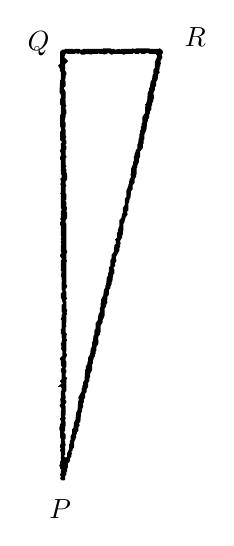
\begin{tikzpicture}[x=0.00883281cm,y=-0.00883281cm]
\fill[even odd rule] (219,60) -- (217,61) -- (205,61) -- (204,60) -- (185,60) -- (184,61) -- (182,61) -- (180,60) -- (179,61) -- (164,61) -- (163,62) -- (161,61) -- (155,62) -- (154,61) -- (149,61) -- (148,60) -- (138,60) -- (137,61) -- (109,61) -- (108,62) -- (105,62) -- (104,61) -- (97,61) -- (96,62) -- (94,61) -- (83,61) -- (82,62) -- (79,62) -- (76,65) -- (76,82) -- (73,85) -- (76,90) -- (76,93) -- (77,94) -- (77,105) -- (76,106) -- (75,123) -- (77,127) -- (77,132) -- (76,133) -- (76,141) -- (77,142) -- (77,155) -- (76,156) -- (76,173) -- (77,174) -- (77,179) -- (76,180) -- (76,192) -- (78,194) -- (78,196) -- (77,197) -- (77,205) -- (76,206) -- (76,209) -- (77,210) -- (77,215) -- (76,216) -- (76,220) -- (77,221) -- (77,241) -- (78,242) -- (78,246) -- (76,248) -- (77,250) -- (77,254) -- (76,255) -- (77,257) -- (77,267) -- (76,269) -- (77,270) -- (77,290) -- (78,291) -- (78,293) -- (77,294) -- (77,304) -- (76,305) -- (77,307) -- (77,309) -- (76,310) -- (76,314) -- (77,315) -- (77,330) -- (78,331) -- (77,333) -- (77,335) -- (78,336) -- (77,338) -- (77,340) -- (78,341) -- (77,343) -- (77,352) -- (78,354) -- (76,357) -- (76,359) -- (78,362) -- (78,364) -- (77,365) -- (77,380) -- (78,381) -- (77,388) -- (78,389) -- (78,393) -- (79,394) -- (78,396) -- (78,407) -- (79,408) -- (79,410) -- (77,413) -- (77,419) -- (78,420) -- (80,427) -- (78,429) -- (78,439) -- (79,440) -- (79,442) -- (78,443) -- (78,447) -- (77,448) -- (77,450) -- (78,451) -- (78,463) -- (77,464) -- (77,470) -- (78,471) -- (78,476) -- (79,477) -- (78,483) -- (77,484) -- (77,487) -- (78,488) -- (77,492) -- (79,495) -- (79,502) -- (76,505) -- (76,508) -- (77,509) -- (77,516) -- (79,518) -- (79,519) -- (77,521) -- (77,525) -- (78,526) -- (78,536) -- (76,538) -- (76,540) -- (77,540) -- (78,542) -- (73,546) -- (74,547) -- (76,546) -- (78,548) -- (78,552) -- (77,553) -- (77,563) -- (76,564) -- (77,571) -- (75,573) -- (78,579) -- (77,581) -- (77,591) -- (76,592) -- (76,594) -- (77,595) -- (77,599) -- (76,600) -- (76,603) -- (75,604) -- (75,609) -- (76,610) -- (76,620) -- (77,621) -- (77,629) -- (76,630) -- (76,634) -- (77,635) -- (76,637) -- (76,639) -- (77,640) -- (77,653) -- (76,654) -- (76,658) -- (75,659) -- (75,661) -- (76,662) -- (76,664) -- (78,666) -- (77,668) -- (77,671) -- (76,672) -- (76,674) -- (77,675) -- (76,679) -- (78,681) -- (82,681) -- (83,680) -- (83,675) -- (85,673) -- (85,669) -- (86,668) -- (86,664) -- (87,663) -- (87,657) -- (89,655) -- (90,653) -- (90,650) -- (92,647) -- (92,644) -- (93,643) -- (92,640) -- (94,638) -- (94,636) -- (96,634) -- (96,626) -- (99,619) -- (99,615) -- (100,614) -- (100,612) -- (102,610) -- (102,605) -- (104,602) -- (103,599) -- (105,597) -- (106,584) -- (107,583) -- (108,577) -- (109,576) -- (109,570) -- (110,569) -- (110,565) -- (112,562) -- (112,556) -- (114,554) -- (114,550) -- (116,547) -- (116,541) -- (118,538) -- (118,534) -- (119,533) -- (119,528) -- (122,522) -- (122,514) -- (123,513) -- (123,508) -- (124,507) -- (124,505) -- (126,503) -- (126,500) -- (127,499) -- (127,496) -- (128,495) -- (128,489) -- (131,485) -- (131,479) -- (130,477) -- (131,476) -- (131,474) -- (133,472) -- (133,469) -- (134,468) -- (134,459) -- (137,454) -- (137,451) -- (140,444) -- (140,434) -- (142,431) -- (142,429) -- (144,425) -- (143,422) -- (144,421) -- (144,417) -- (146,414) -- (146,407) -- (148,405) -- (148,403) -- (150,399) -- (150,396) -- (151,395) -- (152,386) -- (154,383) -- (154,378) -- (153,377) -- (153,375) -- (155,373) -- (155,369) -- (157,365) -- (156,363) -- (156,360) -- (161,351) -- (161,347) -- (162,346) -- (162,342) -- (163,341) -- (162,337) -- (165,332) -- (165,329) -- (166,328) -- (166,323) -- (167,322) -- (167,312) -- (168,311) -- (170,303) -- (173,299) -- (172,295) -- (174,293) -- (174,283) -- (175,282) -- (176,276) -- (177,275) -- (178,265) -- (180,263) -- (180,257) -- (183,253) -- (183,248) -- (185,245) -- (185,242) -- (186,241) -- (186,232) -- (187,231) -- (187,228) -- (189,224) -- (189,219) -- (191,216) -- (191,208) -- (195,203) -- (195,198) -- (196,197) -- (196,192) -- (197,191) -- (197,184) -- (200,177) -- (201,166) -- (202,165) -- (202,162) -- (204,160) -- (204,155) -- (205,154) -- (205,151) -- (207,148) -- (207,143) -- (208,142) -- (208,139) -- (210,136) -- (210,133) -- (211,132) -- (210,124) -- (212,120) -- (212,116) -- (214,114) -- (214,108) -- (216,105) -- (217,97) -- (219,95) -- (218,91) -- (219,90) -- (219,87) -- (220,86) -- (220,83) -- (221,82) -- (220,79) -- (223,73) -- (222,69) -- (224,66) -- (223,63) -- cycle
(213,68) -- (215,70) -- (215,73) -- (212,80) -- (212,88) -- (210,91) -- (210,97) -- (209,98) -- (208,105) -- (206,108) -- (205,116) -- (204,117) -- (204,121) -- (202,123) -- (201,136) -- (200,137) -- (200,139) -- (198,141) -- (199,143) -- (198,145) -- (198,153) -- (194,159) -- (194,167) -- (193,168) -- (193,172) -- (192,173) -- (192,177) -- (191,178) -- (191,182) -- (190,183) -- (190,188) -- (189,189) -- (188,197) -- (187,198) -- (187,204) -- (185,206) -- (184,210) -- (183,211) -- (183,214) -- (182,215) -- (182,222) -- (181,223) -- (181,226) -- (178,233) -- (178,240) -- (177,241) -- (178,245) -- (176,248) -- (176,250) -- (175,251) -- (175,255) -- (174,256) -- (174,258) -- (171,265) -- (171,274) -- (169,276) -- (169,285) -- (166,290) -- (166,297) -- (165,298) -- (164,304) -- (161,307) -- (161,316) -- (160,317) -- (160,319) -- (159,320) -- (159,324) -- (158,325) -- (158,332) -- (155,335) -- (156,337) -- (156,341) -- (154,343) -- (153,353) -- (150,357) -- (150,362) -- (148,365) -- (148,373) -- (146,375) -- (146,382) -- (145,383) -- (145,386) -- (143,390) -- (142,400) -- (141,401) -- (141,404) -- (139,407) -- (138,415) -- (135,421) -- (135,426) -- (134,427) -- (134,432) -- (133,433) -- (133,439) -- (131,443) -- (130,451) -- (127,455) -- (127,463) -- (125,466) -- (125,472) -- (124,473) -- (123,481) -- (122,482) -- (122,488) -- (120,492) -- (119,500) -- (116,505) -- (116,510) -- (115,511) -- (115,514) -- (113,517) -- (113,521) -- (112,522) -- (111,537) -- (109,540) -- (109,544) -- (108,545) -- (108,548) -- (107,549) -- (107,553) -- (102,562) -- (103,566) -- (102,567) -- (101,580) -- (99,584) -- (98,594) -- (96,598) -- (95,606) -- (93,608) -- (93,614) -- (91,618) -- (91,623) -- (90,624) -- (90,628) -- (89,629) -- (89,636) -- (86,642) -- (86,647) -- (85,648) -- (83,648) -- (82,647) -- (82,645) -- (83,644) -- (83,632) -- (84,631) -- (84,629) -- (83,628) -- (83,625) -- (82,623) -- (84,621) -- (84,615) -- (82,613) -- (82,611) -- (83,610) -- (83,604) -- (84,603) -- (84,597) -- (83,596) -- (83,594) -- (84,593) -- (84,591) -- (83,590) -- (83,588) -- (84,587) -- (84,575) -- (83,574) -- (83,572) -- (85,569) -- (85,567) -- (83,565) -- (84,563) -- (83,555) -- (85,552) -- (85,536) -- (86,535) -- (86,534) -- (84,532) -- (84,527) -- (85,526) -- (85,523) -- (84,522) -- (84,519) -- (85,518) -- (85,510) -- (84,509) -- (84,505) -- (86,501) -- (84,497) -- (85,495) -- (85,481) -- (86,480) -- (85,478) -- (85,473) -- (86,471) -- (84,469) -- (84,461) -- (85,460) -- (84,455) -- (85,454) -- (85,443) -- (86,442) -- (85,440) -- (86,438) -- (86,436) -- (85,435) -- (85,424) -- (84,423) -- (84,422) -- (86,420) -- (85,418) -- (85,410) -- (84,409) -- (84,406) -- (86,403) -- (86,401) -- (85,400) -- (85,367) -- (86,366) -- (85,364) -- (85,355) -- (86,354) -- (86,351) -- (85,350) -- (85,312) -- (84,311) -- (84,307) -- (86,304) -- (86,296) -- (85,295) -- (86,289) -- (85,288) -- (85,281) -- (84,280) -- (84,278) -- (85,277) -- (85,270) -- (84,269) -- (84,259) -- (85,257) -- (84,256) -- (84,251) -- (86,249) -- (86,240) -- (85,239) -- (85,234) -- (84,233) -- (84,231) -- (85,230) -- (84,228) -- (84,218) -- (85,217) -- (85,215) -- (84,214) -- (84,206) -- (85,205) -- (85,201) -- (84,200) -- (84,198) -- (85,197) -- (85,193) -- (84,192) -- (84,189) -- (85,187) -- (84,186) -- (84,177) -- (83,176) -- (83,174) -- (84,173) -- (84,167) -- (82,165) -- (83,163) -- (83,160) -- (84,159) -- (84,155) -- (85,154) -- (85,149) -- (84,148) -- (84,144) -- (85,142) -- (84,141) -- (84,135) -- (83,134) -- (84,132) -- (84,123) -- (81,117) -- (84,114) -- (84,108) -- (83,107) -- (83,104) -- (84,103) -- (84,99) -- (85,98) -- (85,95) -- (83,92) -- (83,83) -- (87,79) -- (87,78) -- (82,73) -- (82,72) -- (83,71) -- (83,69) -- (85,67) -- (87,68) -- (97,68) -- (98,67) -- (102,68) -- (104,67) -- (106,69) -- (112,69) -- (113,68) -- (121,69) -- (122,68) -- (130,68) -- (131,67) -- (133,68) -- (138,68) -- (139,69) -- (143,68) -- (144,67) -- (146,67) -- (149,69) -- (151,69) -- (152,68) -- (165,68) -- (166,69) -- (169,69) -- (170,68) -- (180,68) -- (181,67) -- (183,67) -- (184,68) -- (189,68) -- (190,67) -- (192,67) -- (193,68) -- (198,68) -- (199,67) -- (203,67) -- (204,68) -- cycle;
\node[inner sep=0pt] at (45,53) {$Q$};
\node[inner sep=0pt] at (270,44) {$R$};
\node[inner sep=0pt] at (76,722) {$P$};
\end{tikzpicture}
\end{center}

\noindent Aus 1) folgt leicht, dass f\"ur ein unendlich kleines $P$, wenn $Q=90^{0}$:

\[
R = 90^{0} - gPQ\,.\,P.
\]

\begin{center}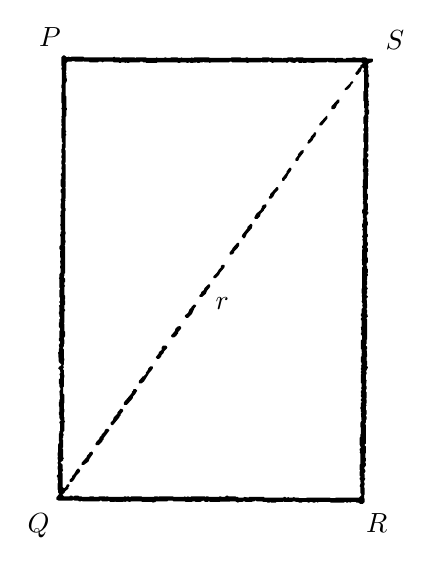
\begin{tikzpicture}[x=0.00801815cm,y=-0.00801815cm]
\fill[even odd rule] (81,75) -- (78,78) -- (78,91) -- (79,92) -- (79,94) -- (78,95) -- (78,97) -- (79,98) -- (79,121) -- (78,122) -- (78,126) -- (79,127) -- (79,133) -- (78,134) -- (78,150) -- (79,151) -- (79,158) -- (78,159) -- (79,161) -- (79,171) -- (78,172) -- (79,175) -- (78,176) -- (78,181) -- (79,183) -- (78,184) -- (78,186) -- (79,187) -- (79,190) -- (78,191) -- (78,206) -- (79,207) -- (79,212) -- (80,213) -- (80,215) -- (79,216) -- (79,223) -- (78,224) -- (78,229) -- (79,230) -- (79,233) -- (78,234) -- (78,237) -- (79,238) -- (79,241) -- (78,242) -- (78,247) -- (79,248) -- (78,255) -- (79,256) -- (79,260) -- (77,264) -- (78,266) -- (78,271) -- (77,272) -- (77,282) -- (79,285) -- (79,286) -- (77,288) -- (77,292) -- (78,293) -- (78,302) -- (77,303) -- (78,309) -- (77,310) -- (77,317) -- (78,318) -- (78,321) -- (77,322) -- (77,328) -- (76,329) -- (77,331) -- (77,342) -- (76,344) -- (77,345) -- (77,351) -- (78,352) -- (78,354) -- (77,355) -- (77,358) -- (76,359) -- (76,361) -- (77,362) -- (77,375) -- (75,378) -- (75,382) -- (77,384) -- (76,386) -- (76,395) -- (77,396) -- (77,400) -- (76,401) -- (77,408) -- (76,409) -- (76,412) -- (77,413) -- (77,419) -- (75,422) -- (75,427) -- (74,428) -- (75,430) -- (75,443) -- (76,444) -- (76,446) -- (75,447) -- (75,458) -- (76,459) -- (76,464) -- (75,465) -- (75,467) -- (76,468) -- (76,470) -- (74,472) -- (75,474) -- (75,481) -- (74,482) -- (74,485) -- (75,486) -- (75,489) -- (76,490) -- (76,492) -- (75,493) -- (75,498) -- (74,499) -- (74,505) -- (76,508) -- (76,511) -- (75,512) -- (75,523) -- (74,524) -- (74,527) -- (76,529) -- (76,531) -- (74,534) -- (75,539) -- (74,540) -- (74,545) -- (73,546) -- (74,561) -- (78,565) -- (78,566) -- (76,568) -- (75,568) -- (73,571) -- (76,574) -- (76,576) -- (77,577) -- (75,581) -- (76,583) -- (76,587) -- (74,589) -- (74,595) -- (75,596) -- (75,600) -- (77,604) -- (75,608) -- (76,620) -- (75,621) -- (75,624) -- (74,625) -- (74,631) -- (75,632) -- (75,640) -- (74,641) -- (74,644) -- (75,645) -- (75,650) -- (77,654) -- (75,656) -- (75,658) -- (76,659) -- (76,670) -- (75,671) -- (75,674) -- (74,675) -- (74,686) -- (75,688) -- (73,692) -- (73,704) -- (72,705) -- (72,709) -- (73,710) -- (72,712) -- (72,715) -- (73,716) -- (73,719) -- (72,720) -- (72,722) -- (73,723) -- (73,726) -- (72,727) -- (72,731) -- (73,732) -- (73,739) -- (71,741) -- (71,743) -- (72,744) -- (72,748) -- (73,749) -- (73,753) -- (72,754) -- (72,763) -- (73,764) -- (73,768) -- (74,769) -- (74,771) -- (70,776) -- (70,779) -- (74,781) -- (95,781) -- (96,780) -- (98,780) -- (99,781) -- (105,781) -- (106,782) -- (109,782) -- (110,781) -- (112,782) -- (138,782) -- (139,781) -- (142,781) -- (143,782) -- (151,782) -- (153,781) -- (156,783) -- (162,783) -- (163,782) -- (165,783) -- (176,783) -- (177,782) -- (179,783) -- (181,782) -- (184,782) -- (185,783) -- (187,783) -- (188,782) -- (205,782) -- (206,783) -- (222,783) -- (223,784) -- (227,783) -- (228,782) -- (246,782) -- (247,781) -- (255,781) -- (256,782) -- (274,782) -- (275,783) -- (285,783) -- (286,782) -- (290,782) -- (291,783) -- (298,783) -- (302,781) -- (304,781) -- (306,783) -- (310,783) -- (311,782) -- (313,782) -- (314,783) -- (354,782) -- (358,784) -- (360,783) -- (365,783) -- (366,782) -- (369,782) -- (370,783) -- (380,783) -- (381,782) -- (384,782) -- (385,781) -- (387,781) -- (388,782) -- (397,782) -- (398,783) -- (404,783) -- (405,784) -- (408,784) -- (409,783) -- (411,784) -- (418,784) -- (419,783) -- (429,783) -- (430,782) -- (432,783) -- (444,783) -- (445,782) -- (449,782) -- (450,783) -- (454,783) -- (455,784) -- (459,784) -- (460,783) -- (468,783) -- (469,784) -- (471,784) -- (472,783) -- (476,783) -- (477,784) -- (480,784) -- (481,783) -- (483,783) -- (484,784) -- (486,783) -- (504,783) -- (505,784) -- (526,784) -- (527,783) -- (529,783) -- (530,784) -- (532,784) -- (533,783) -- (537,784) -- (538,783) -- (545,783) -- (546,784) -- (549,784) -- (552,786) -- (556,786) -- (559,783) -- (559,778) -- (558,777) -- (558,772) -- (559,771) -- (559,761) -- (558,760) -- (558,757) -- (559,756) -- (559,753) -- (558,752) -- (558,750) -- (560,746) -- (559,745) -- (559,740) -- (558,738) -- (560,735) -- (560,733) -- (558,729) -- (561,725) -- (561,722) -- (560,721) -- (560,719) -- (561,718) -- (561,714) -- (560,713) -- (560,706) -- (561,705) -- (561,695) -- (559,693) -- (559,692) -- (561,690) -- (561,661) -- (560,660) -- (560,658) -- (561,657) -- (561,653) -- (562,652) -- (562,648) -- (561,647) -- (561,645) -- (562,644) -- (562,638) -- (561,637) -- (561,631) -- (562,630) -- (561,628) -- (562,626) -- (562,621) -- (561,620) -- (562,618) -- (562,609) -- (561,608) -- (561,605) -- (562,604) -- (562,600) -- (561,599) -- (562,590) -- (561,589) -- (561,581) -- (562,580) -- (562,578) -- (561,576) -- (564,570) -- (564,569) -- (562,567) -- (563,565) -- (563,560) -- (562,559) -- (562,553) -- (563,552) -- (562,541) -- (563,540) -- (563,537) -- (561,535) -- (561,533) -- (562,532) -- (562,526) -- (563,525) -- (563,494) -- (562,493) -- (562,491) -- (564,489) -- (563,485) -- (562,484) -- (563,482) -- (563,479) -- (562,478) -- (562,476) -- (563,475) -- (562,460) -- (564,458) -- (564,457) -- (562,455) -- (562,453) -- (563,452) -- (563,449) -- (562,447) -- (564,445) -- (562,441) -- (562,439) -- (563,438) -- (563,433) -- (562,431) -- (563,430) -- (563,425) -- (564,424) -- (564,422) -- (563,421) -- (564,419) -- (564,414) -- (563,413) -- (563,410) -- (562,409) -- (562,405) -- (564,403) -- (564,396) -- (563,395) -- (563,387) -- (564,386) -- (564,381) -- (563,380) -- (563,377) -- (564,376) -- (564,372) -- (563,371) -- (563,363) -- (564,362) -- (564,359) -- (563,358) -- (563,345) -- (564,344) -- (564,339) -- (563,338) -- (563,333) -- (562,332) -- (562,329) -- (565,325) -- (565,324) -- (563,322) -- (564,320) -- (564,310) -- (563,309) -- (563,304) -- (564,303) -- (564,295) -- (563,294) -- (563,287) -- (564,286) -- (564,266) -- (565,265) -- (565,262) -- (564,261) -- (565,259) -- (565,255) -- (563,253) -- (564,251) -- (564,245) -- (565,244) -- (565,241) -- (563,239) -- (563,237) -- (565,234) -- (565,232) -- (563,230) -- (563,228) -- (565,225) -- (565,217) -- (564,216) -- (564,213) -- (565,212) -- (565,198) -- (564,197) -- (565,195) -- (565,189) -- (564,188) -- (564,181) -- (565,180) -- (564,177) -- (565,176) -- (565,172) -- (564,170) -- (566,167) -- (566,162) -- (565,161) -- (565,155) -- (566,154) -- (565,150) -- (566,148) -- (565,147) -- (565,144) -- (564,143) -- (564,141) -- (565,140) -- (565,136) -- (564,135) -- (565,131) -- (564,130) -- (564,128) -- (566,124) -- (566,119) -- (565,118) -- (565,109) -- (566,108) -- (566,106) -- (565,105) -- (565,99) -- (564,98) -- (564,95) -- (565,94) -- (564,89) -- (566,87) -- (570,86) -- (572,84) -- (572,81) -- (571,80) -- (563,80) -- (560,78) -- (555,78) -- (554,79) -- (545,79) -- (544,78) -- (540,78) -- (539,79) -- (530,79) -- (529,80) -- (525,80) -- (524,79) -- (514,79) -- (513,80) -- (511,79) -- (462,79) -- (461,78) -- (450,78) -- (449,79) -- (446,79) -- (445,78) -- (437,78) -- (436,79) -- (430,79) -- (429,80) -- (427,79) -- (413,79) -- (412,78) -- (410,79) -- (408,79) -- (407,78) -- (397,78) -- (396,79) -- (374,79) -- (373,78) -- (371,78) -- (370,79) -- (363,79) -- (362,78) -- (348,78) -- (347,79) -- (313,79) -- (312,78) -- (289,78) -- (288,79) -- (286,79) -- (285,78) -- (283,79) -- (270,79) -- (269,78) -- (267,79) -- (263,79) -- (262,78) -- (252,78) -- (251,79) -- (245,79) -- (244,78) -- (242,78) -- (241,79) -- (231,79) -- (229,78) -- (228,79) -- (213,79) -- (212,78) -- (197,78) -- (195,79) -- (194,78) -- (174,78) -- (173,79) -- (171,79) -- (170,78) -- (163,78) -- (162,77) -- (160,78) -- (114,78) -- (113,77) -- (94,77) -- (93,78) -- (89,77) -- (87,78) -- (83,75) -- cycle
(88,85) -- (94,85) -- (95,84) -- (99,84) -- (100,85) -- (111,85) -- (113,84) -- (114,85) -- (122,85) -- (123,86) -- (136,86) -- (137,85) -- (142,85) -- (143,86) -- (145,85) -- (160,85) -- (161,86) -- (169,86) -- (170,87) -- (172,87) -- (173,86) -- (178,86) -- (179,87) -- (181,86) -- (183,87) -- (185,87) -- (186,86) -- (202,86) -- (203,85) -- (207,85) -- (208,86) -- (212,86) -- (213,87) -- (229,87) -- (230,86) -- (262,86) -- (263,87) -- (266,87) -- (267,86) -- (276,86) -- (277,87) -- (279,87) -- (280,86) -- (282,86) -- (283,87) -- (293,86) -- (294,87) -- (297,87) -- (298,86) -- (302,86) -- (303,85) -- (305,86) -- (312,86) -- (313,87) -- (315,86) -- (344,86) -- (345,85) -- (348,85) -- (349,86) -- (371,86) -- (372,87) -- (374,87) -- (375,86) -- (394,86) -- (395,85) -- (397,86) -- (405,86) -- (406,85) -- (409,85) -- (413,87) -- (415,86) -- (434,86) -- (436,87) -- (439,85) -- (441,85) -- (442,86) -- (448,87) -- (451,85) -- (453,85) -- (455,87) -- (459,87) -- (460,86) -- (462,87) -- (466,87) -- (467,86) -- (479,87) -- (480,86) -- (498,86) -- (499,85) -- (501,85) -- (502,86) -- (511,86) -- (512,87) -- (514,87) -- (515,86) -- (554,86) -- (556,88) -- (552,91) -- (552,93) -- (548,97) -- (548,98) -- (544,103) -- (544,104) -- (546,106) -- (547,106) -- (550,104) -- (550,103) -- (553,100) -- (554,96) -- (556,94) -- (558,96) -- (558,98) -- (557,99) -- (557,101) -- (558,102) -- (558,131) -- (557,132) -- (557,147) -- (558,148) -- (558,158) -- (559,159) -- (559,162) -- (558,163) -- (559,165) -- (559,169) -- (557,173) -- (557,183) -- (558,184) -- (558,190) -- (557,191) -- (557,194) -- (558,195) -- (558,198) -- (557,199) -- (557,212) -- (558,213) -- (558,221) -- (557,222) -- (557,238) -- (556,239) -- (556,249) -- (557,250) -- (557,255) -- (556,256) -- (556,259) -- (557,260) -- (557,271) -- (556,272) -- (556,282) -- (555,283) -- (556,285) -- (556,300) -- (557,301) -- (556,303) -- (557,305) -- (556,307) -- (556,310) -- (557,311) -- (557,318) -- (555,320) -- (555,325) -- (556,326) -- (556,332) -- (557,333) -- (557,335) -- (556,336) -- (556,341) -- (555,342) -- (555,347) -- (556,348) -- (556,350) -- (555,351) -- (556,353) -- (556,360) -- (555,361) -- (555,363) -- (556,364) -- (556,366) -- (555,367) -- (556,369) -- (556,376) -- (555,377) -- (555,380) -- (556,382) -- (555,383) -- (555,398) -- (554,399) -- (555,401) -- (555,407) -- (556,408) -- (556,410) -- (555,411) -- (555,444) -- (554,445) -- (554,452) -- (555,453) -- (555,455) -- (554,456) -- (555,458) -- (555,463) -- (554,465) -- (556,469) -- (555,471) -- (556,475) -- (554,477) -- (554,484) -- (553,485) -- (553,488) -- (554,489) -- (554,491) -- (553,492) -- (553,494) -- (554,495) -- (554,505) -- (553,506) -- (554,514) -- (553,515) -- (553,517) -- (555,520) -- (555,525) -- (553,527) -- (553,540) -- (554,541) -- (554,544) -- (555,546) -- (554,547) -- (554,552) -- (553,553) -- (553,561) -- (554,562) -- (554,566) -- (553,567) -- (554,569) -- (553,571) -- (553,573) -- (554,574) -- (553,576) -- (553,578) -- (554,579) -- (553,581) -- (553,594) -- (554,595) -- (554,601) -- (553,602) -- (554,604) -- (554,606) -- (553,607) -- (553,610) -- (554,612) -- (553,613) -- (553,616) -- (554,617) -- (554,619) -- (553,620) -- (553,622) -- (554,623) -- (554,625) -- (553,626) -- (553,632) -- (552,633) -- (552,635) -- (553,636) -- (553,640) -- (554,641) -- (553,643) -- (554,654) -- (552,658) -- (552,664) -- (553,665) -- (553,675) -- (552,676) -- (552,680) -- (551,681) -- (551,692) -- (553,697) -- (551,699) -- (551,701) -- (552,702) -- (551,704) -- (552,706) -- (552,723) -- (551,724) -- (551,732) -- (552,733) -- (551,735) -- (551,741) -- (552,742) -- (552,744) -- (551,745) -- (551,747) -- (552,748) -- (552,751) -- (553,752) -- (551,758) -- (552,759) -- (552,768) -- (554,772) -- (550,776) -- (513,776) -- (512,777) -- (505,777) -- (504,776) -- (467,776) -- (466,777) -- (455,777) -- (454,776) -- (448,776) -- (447,775) -- (445,776) -- (439,776) -- (438,775) -- (436,776) -- (434,776) -- (433,775) -- (431,775) -- (430,776) -- (400,776) -- (399,775) -- (376,775) -- (375,776) -- (368,775) -- (367,776) -- (359,776) -- (358,775) -- (355,775) -- (354,774) -- (343,774) -- (342,773) -- (340,773) -- (337,775) -- (332,775) -- (331,774) -- (329,774) -- (328,775) -- (312,775) -- (311,774) -- (308,774) -- (307,775) -- (305,774) -- (284,774) -- (283,775) -- (280,775) -- (279,774) -- (277,775) -- (275,775) -- (274,774) -- (272,775) -- (256,775) -- (255,774) -- (233,774) -- (232,775) -- (230,774) -- (226,774) -- (225,775) -- (206,775) -- (205,774) -- (189,774) -- (188,775) -- (186,775) -- (185,774) -- (183,774) -- (182,775) -- (180,774) -- (178,774) -- (177,775) -- (153,775) -- (152,774) -- (150,774) -- (148,775) -- (147,774) -- (138,774) -- (137,775) -- (130,775) -- (129,774) -- (123,774) -- (122,775) -- (111,775) -- (110,774) -- (106,774) -- (105,773) -- (99,773) -- (98,774) -- (96,774) -- (95,773) -- (92,773) -- (91,774) -- (82,774) -- (80,772) -- (80,771) -- (84,767) -- (84,766) -- (89,762) -- (89,760) -- (91,757) -- (90,755) -- (87,755) -- (85,759) -- (83,761) -- (82,761) -- (80,759) -- (80,738) -- (79,736) -- (81,732) -- (80,731) -- (80,724) -- (77,721) -- (77,720) -- (81,717) -- (81,715) -- (82,714) -- (81,712) -- (81,700) -- (80,699) -- (80,697) -- (81,696) -- (81,685) -- (80,684) -- (80,682) -- (81,681) -- (81,678) -- (82,677) -- (81,675) -- (81,672) -- (83,670) -- (83,657) -- (84,656) -- (83,654) -- (83,649) -- (82,648) -- (82,641) -- (83,640) -- (83,636) -- (82,635) -- (82,627) -- (83,626) -- (83,613) -- (81,611) -- (81,601) -- (82,600) -- (82,586) -- (83,585) -- (83,582) -- (82,581) -- (82,574) -- (81,573) -- (81,571) -- (82,570) -- (81,566) -- (82,565) -- (82,559) -- (83,558) -- (83,556) -- (82,555) -- (82,541) -- (81,540) -- (81,537) -- (82,536) -- (82,533) -- (83,532) -- (83,526) -- (82,525) -- (82,523) -- (84,520) -- (84,513) -- (83,512) -- (83,501) -- (82,500) -- (83,498) -- (83,481) -- (84,480) -- (84,478) -- (83,477) -- (83,471) -- (84,470) -- (84,464) -- (83,463) -- (84,461) -- (84,456) -- (83,455) -- (83,442) -- (84,440) -- (83,439) -- (83,435) -- (84,434) -- (84,429) -- (82,427) -- (82,425) -- (83,424) -- (83,421) -- (84,420) -- (84,378) -- (83,376) -- (84,375) -- (84,372) -- (85,371) -- (85,369) -- (84,368) -- (84,359) -- (85,358) -- (85,355) -- (84,354) -- (84,322) -- (85,321) -- (85,318) -- (84,317) -- (84,306) -- (85,305) -- (84,303) -- (85,301) -- (85,286) -- (84,285) -- (85,283) -- (85,274) -- (84,273) -- (85,271) -- (85,248) -- (84,247) -- (84,245) -- (85,244) -- (85,226) -- (84,225) -- (84,222) -- (85,221) -- (85,202) -- (86,201) -- (85,199) -- (85,197) -- (86,196) -- (85,194) -- (85,172) -- (86,171) -- (86,162) -- (87,161) -- (87,159) -- (86,158) -- (86,140) -- (85,139) -- (85,119) -- (87,115) -- (87,112) -- (86,111) -- (86,107) -- (85,106) -- (86,104) -- (85,100) -- (86,99) -- (86,87) -- cycle
(105,730) -- (104,730) -- (102,732) -- (98,739) -- (95,742) -- (95,744) -- (91,748) -- (91,750) -- (92,751) -- (95,751) -- (98,748) -- (102,741) -- (107,736) -- (108,733) -- cycle
(126,703) -- (122,705) -- (122,706) -- (119,709) -- (118,712) -- (110,721) -- (110,724) -- (114,724) -- (121,719) -- (123,714) -- (128,707) -- (128,705) -- cycle
(152,667) -- (149,667) -- (147,669) -- (146,672) -- (142,676) -- (142,677) -- (139,680) -- (138,683) -- (134,687) -- (132,691) -- (133,693) -- (137,693) -- (143,687) -- (143,686) -- (145,684) -- (145,682) -- (154,670) -- (154,669) -- cycle
(175,636) -- (172,635) -- (167,641) -- (167,643) -- (161,649) -- (160,653) -- (156,657) -- (156,659) -- (158,661) -- (160,661) -- (170,649) -- (170,648) -- (172,646) -- (172,644) -- (176,639) -- (176,637) -- cycle
(196,604) -- (193,604) -- (192,605) -- (192,606) -- (190,608) -- (190,610) -- (178,624) -- (177,626) -- (177,628) -- (178,629) -- (182,629) -- (191,619) -- (192,615) -- (195,612) -- (198,607) -- (198,606) -- cycle
(222,568) -- (219,568) -- (216,571) -- (215,574) -- (212,578) -- (212,580) -- (208,584) -- (207,584) -- (201,591) -- (201,594) -- (202,595) -- (205,595) -- (209,592) -- (217,579) -- (222,573) -- (223,571) -- (223,569) -- cycle
(245,536) -- (243,535) -- (239,535) -- (237,538) -- (237,542) -- (233,545) -- (232,548) -- (228,553) -- (228,554) -- (230,556) -- (233,556) -- (236,553) -- (237,550) -- (240,547) -- (241,544) -- (245,540) -- (246,538) -- cycle
(266,504) -- (262,505) -- (259,508) -- (258,512) -- (252,519) -- (252,520) -- (254,522) -- (257,522) -- (261,519) -- (261,518) -- (263,516) -- (263,514) -- (268,508) -- (268,506) -- cycle
(290,470) -- (288,470) -- (284,474) -- (284,475) -- (281,478) -- (279,483) -- (274,487) -- (274,489) -- (276,491) -- (279,491) -- (285,485) -- (289,476) -- (292,472) -- cycle
(313,438) -- (311,438) -- (305,444) -- (304,447) -- (300,450) -- (299,453) -- (297,455) -- (297,457) -- (298,458) -- (301,458) -- (307,453) -- (309,448) -- (314,442) -- (314,439) -- cycle
(336,407) -- (333,407) -- (331,409) -- (331,411) -- (328,414) -- (325,419) -- (319,425) -- (319,427) -- (320,428) -- (323,428) -- (328,423) -- (330,419) -- (336,412) -- (337,410) -- (337,408) -- cycle
(359,372) -- (357,372) -- (349,381) -- (349,382) -- (345,387) -- (345,390) -- (346,391) -- (350,390) -- (352,388) -- (352,386) -- (358,380) -- (358,379) -- (360,377) -- (360,373) -- cycle
(379,342) -- (378,342) -- (373,347) -- (373,349) -- (365,359) -- (364,362) -- (367,365) -- (368,365) -- (370,363) -- (372,358) -- (380,349) -- (381,344) -- cycle
(402,311) -- (398,312) -- (396,314) -- (396,316) -- (394,320) -- (387,326) -- (384,332) -- (385,334) -- (389,334) -- (393,330) -- (394,326) -- (399,321) -- (399,320) -- (403,315) -- (403,312) -- cycle
(421,284) -- (419,284) -- (409,295) -- (409,297) -- (407,299) -- (407,301) -- (408,302) -- (411,302) -- (414,299) -- (417,293) -- (422,288) -- (422,285) -- cycle
(441,253) -- (440,253) -- (437,256) -- (437,257) -- (435,259) -- (435,261) -- (428,270) -- (428,273) -- (429,274) -- (431,274) -- (432,273) -- (432,272) -- (435,269) -- (438,263) -- (442,258) -- (443,255) -- cycle
(462,225) -- (458,226) -- (453,232) -- (453,234) -- (449,239) -- (449,241) -- (450,242) -- (453,242) -- (454,241) -- (455,238) -- (462,229) -- cycle
(481,197) -- (479,197) -- (478,198) -- (478,199) -- (474,203) -- (473,206) -- (469,210) -- (469,212) -- (468,213) -- (469,215) -- (472,214) -- (476,210) -- (478,206) -- (481,203) -- (481,201) -- (482,200) -- (482,198) -- cycle
(499,171) -- (498,171) -- (487,183) -- (487,185) -- (488,186) -- (491,186) -- (500,175) -- (500,172) -- cycle
(518,145) -- (516,145) -- (506,156) -- (506,159) -- (507,160) -- (511,160) -- (513,158) -- (515,153) -- (519,149) -- (519,146) -- cycle
(540,116) -- (538,116) -- (536,118) -- (536,119) -- (527,128) -- (528,130) -- (532,129) -- (536,125) -- (538,121) -- (541,118) -- cycle;
\node[inner sep=0pt] at (60,46) {$P$};
\node[inner sep=0pt] at (607,51) {$S$};
\node[inner sep=0pt] at (333,468) {$r$};
\node[inner sep=0pt] at (42,821) {$Q$};
\node[inner sep=0pt] at (578,816) {$R$};
\end{tikzpicture}
\end{center}

\noindent Eben so, wenn $P,Q,R$ rechte Winkel sind, und $PQ$ unendlich klein, wird:

\[
PSQ = \frac{PQ}{fr},
\]
\[
RQS = gr\,.\,PSQ = \frac{gr}{fr}\cdot PQ,
\]
\[
\begin{aligned}RSQ &= 90^{0} - gr\,.\,RQS = 90^{0} - gr^{2}\,.\,PSQ\\ &= 90^{0} - \frac{gr^{2}}{fr}\cdot PQ,\end{aligned}
\]

\noindent also

\[
PSR = 90^{0} + \frac{1-gr^{2}}{fr}\cdot PQ.
\]

\begin{center}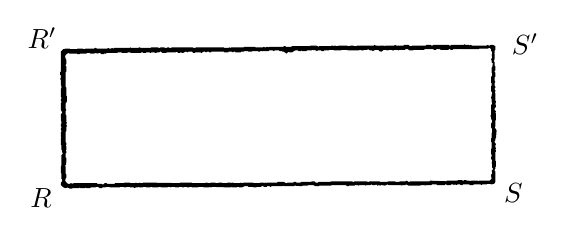
\begin{tikzpicture}[x=0.00787402cm,y=-0.00787402cm]
\fill[even odd rule] (779,77) -- (775,75) -- (771,75) -- (770,76) -- (768,76) -- (767,75) -- (765,76) -- (741,76) -- (739,75) -- (737,76) -- (736,75) -- (731,75) -- (729,74) -- (728,75) -- (708,75) -- (707,76) -- (705,76) -- (704,75) -- (679,75) -- (678,76) -- (676,76) -- (675,75) -- (668,75) -- (667,76) -- (645,76) -- (644,77) -- (641,77) -- (639,75) -- (632,75) -- (631,76) -- (619,76) -- (617,75) -- (616,76) -- (602,76) -- (601,77) -- (599,76) -- (593,76) -- (591,77) -- (590,76) -- (586,76) -- (584,75) -- (583,76) -- (556,76) -- (555,77) -- (551,77) -- (550,76) -- (545,76) -- (544,77) -- (541,77) -- (540,76) -- (526,76) -- (525,77) -- (522,77) -- (520,76) -- (518,77) -- (517,76) -- (515,76) -- (514,77) -- (495,77) -- (494,78) -- (490,76) -- (481,76) -- (480,77) -- (451,77) -- (450,78) -- (441,78) -- (440,77) -- (438,77) -- (437,78) -- (414,78) -- (413,79) -- (411,78) -- (409,79) -- (407,79) -- (406,78) -- (404,79) -- (392,79) -- (391,78) -- (374,78) -- (373,79) -- (353,79) -- (352,80) -- (350,79) -- (348,80) -- (342,80) -- (341,79) -- (296,79) -- (295,80) -- (292,80) -- (291,79) -- (257,79) -- (256,80) -- (253,80) -- (252,79) -- (250,79) -- (249,80) -- (246,80) -- (245,79) -- (239,79) -- (238,80) -- (236,80) -- (235,79) -- (224,79) -- (223,80) -- (207,80) -- (206,79) -- (204,79) -- (203,80) -- (192,80) -- (190,79) -- (189,80) -- (164,80) -- (163,81) -- (161,80) -- (159,81) -- (156,81) -- (155,80) -- (153,81) -- (136,81) -- (135,80) -- (133,80) -- (132,81) -- (118,81) -- (117,82) -- (115,82) -- (114,81) -- (105,81) -- (104,82) -- (93,82) -- (92,81) -- (85,81) -- (84,82) -- (82,82) -- (78,86) -- (78,118) -- (77,119) -- (77,123) -- (78,124) -- (78,128) -- (77,130) -- (78,131) -- (78,140) -- (79,141) -- (79,145) -- (78,146) -- (78,159) -- (79,160) -- (79,162) -- (78,163) -- (78,165) -- (79,166) -- (79,168) -- (78,169) -- (78,180) -- (80,183) -- (80,185) -- (78,187) -- (78,193) -- (79,194) -- (78,196) -- (79,198) -- (79,202) -- (78,203) -- (78,206) -- (79,207) -- (79,209) -- (78,210) -- (78,212) -- (79,213) -- (79,215) -- (78,216) -- (78,223) -- (79,224) -- (78,226) -- (78,236) -- (79,237) -- (79,244) -- (80,245) -- (80,248) -- (81,249) -- (81,251) -- (79,253) -- (79,270) -- (78,271) -- (78,281) -- (79,282) -- (79,291) -- (80,292) -- (80,295) -- (78,298) -- (78,301) -- (81,304) -- (85,306) -- (89,305) -- (93,307) -- (96,307) -- (97,306) -- (107,306) -- (108,305) -- (110,306) -- (117,306) -- (118,305) -- (120,306) -- (125,306) -- (126,305) -- (134,305) -- (135,304) -- (138,304) -- (141,306) -- (144,306) -- (145,305) -- (150,305) -- (151,304) -- (156,304) -- (157,305) -- (173,305) -- (174,304) -- (180,304) -- (181,305) -- (183,305) -- (184,304) -- (189,304) -- (190,305) -- (196,305) -- (197,306) -- (199,305) -- (202,305) -- (203,304) -- (205,305) -- (210,305) -- (211,304) -- (215,304) -- (216,305) -- (222,305) -- (223,304) -- (225,304) -- (226,305) -- (235,305) -- (236,304) -- (239,304) -- (240,305) -- (250,305) -- (251,304) -- (254,304) -- (255,305) -- (257,304) -- (262,304) -- (263,305) -- (268,305) -- (269,304) -- (273,304) -- (274,305) -- (276,305) -- (277,304) -- (281,304) -- (282,305) -- (285,305) -- (286,304) -- (289,304) -- (290,305) -- (299,305) -- (300,304) -- (308,304) -- (309,305) -- (317,305) -- (318,304) -- (320,305) -- (322,304) -- (352,305) -- (354,304) -- (355,305) -- (362,305) -- (363,304) -- (365,304) -- (366,305) -- (370,305) -- (374,303) -- (380,303) -- (381,304) -- (388,304) -- (389,305) -- (393,305) -- (394,304) -- (401,304) -- (402,303) -- (405,303) -- (406,304) -- (410,304) -- (411,303) -- (415,303) -- (416,304) -- (418,303) -- (436,303) -- (437,302) -- (439,303) -- (454,303) -- (455,302) -- (467,303) -- (468,302) -- (476,302) -- (477,301) -- (485,301) -- (489,303) -- (494,303) -- (495,302) -- (514,302) -- (515,301) -- (538,301) -- (540,303) -- (542,303) -- (543,302) -- (552,302) -- (553,301) -- (557,301) -- (558,302) -- (560,301) -- (568,301) -- (570,302) -- (571,301) -- (578,301) -- (579,300) -- (581,301) -- (585,301) -- (587,300) -- (589,302) -- (591,301) -- (593,302) -- (595,301) -- (601,302) -- (605,300) -- (607,301) -- (627,301) -- (628,302) -- (630,301) -- (634,301) -- (635,300) -- (639,302) -- (658,302) -- (659,301) -- (664,301) -- (666,302) -- (667,301) -- (676,301) -- (677,300) -- (684,300) -- (685,301) -- (697,301) -- (698,300) -- (700,300) -- (701,301) -- (707,301) -- (708,300) -- (711,300) -- (712,301) -- (714,300) -- (716,301) -- (718,300) -- (722,300) -- (723,301) -- (726,301) -- (727,300) -- (737,300) -- (738,301) -- (743,301) -- (744,300) -- (755,300) -- (757,301) -- (758,300) -- (765,300) -- (766,299) -- (771,299) -- (772,300) -- (774,300) -- (775,299) -- (777,299) -- (779,296) -- (779,279) -- (778,278) -- (778,276) -- (779,275) -- (779,272) -- (780,271) -- (780,263) -- (779,262) -- (779,248) -- (780,247) -- (780,245) -- (779,244) -- (780,242) -- (779,240) -- (779,237) -- (780,235) -- (778,232) -- (778,230) -- (779,229) -- (779,226) -- (780,225) -- (781,213) -- (778,208) -- (779,206) -- (779,197) -- (780,196) -- (780,186) -- (779,185) -- (780,182) -- (778,180) -- (778,177) -- (780,175) -- (780,172) -- (779,171) -- (780,166) -- (779,165) -- (779,153) -- (778,152) -- (779,150) -- (779,148) -- (778,147) -- (778,145) -- (779,144) -- (779,142) -- (778,141) -- (778,136) -- (779,135) -- (778,133) -- (778,127) -- (779,126) -- (779,120) -- (778,119) -- (778,117) -- (779,116) -- (779,110) -- (778,109) -- (778,103) -- (777,102) -- (777,99) -- (778,98) -- (778,90) -- (777,88) -- (778,87) -- (778,84) -- (779,83) -- cycle
(774,87) -- (774,90) -- (773,91) -- (774,96) -- (772,98) -- (773,100) -- (773,103) -- (775,105) -- (774,111) -- (773,112) -- (773,120) -- (774,121) -- (774,124) -- (772,127) -- (772,136) -- (773,137) -- (773,141) -- (772,142) -- (772,149) -- (774,152) -- (772,161) -- (773,162) -- (773,167) -- (774,169) -- (772,173) -- (772,188) -- (771,190) -- (772,191) -- (772,194) -- (774,197) -- (773,201) -- (772,202) -- (772,208) -- (774,211) -- (774,216) -- (773,217) -- (773,225) -- (772,226) -- (772,231) -- (773,232) -- (773,242) -- (772,243) -- (772,251) -- (773,252) -- (773,255) -- (772,256) -- (772,259) -- (774,261) -- (773,266) -- (774,267) -- (774,273) -- (775,274) -- (775,276) -- (773,278) -- (774,282) -- (772,285) -- (773,291) -- (770,294) -- (753,294) -- (752,295) -- (750,294) -- (740,294) -- (738,295) -- (737,294) -- (733,294) -- (732,293) -- (729,293) -- (728,294) -- (726,294) -- (725,293) -- (719,293) -- (718,294) -- (701,294) -- (700,295) -- (674,294) -- (673,295) -- (642,295) -- (641,296) -- (639,296) -- (636,294) -- (634,295) -- (625,295) -- (624,296) -- (618,296) -- (617,295) -- (606,295) -- (605,296) -- (593,296) -- (592,295) -- (576,295) -- (575,296) -- (573,296) -- (572,295) -- (552,295) -- (551,296) -- (549,296) -- (548,295) -- (514,295) -- (513,296) -- (494,296) -- (493,297) -- (489,297) -- (487,295) -- (483,295) -- (482,296) -- (466,296) -- (465,297) -- (458,297) -- (457,296) -- (454,296) -- (453,297) -- (444,297) -- (443,298) -- (441,298) -- (438,296) -- (428,296) -- (427,297) -- (411,297) -- (410,298) -- (408,297) -- (406,298) -- (404,297) -- (400,297) -- (399,298) -- (389,298) -- (388,297) -- (373,297) -- (372,298) -- (370,298) -- (369,297) -- (367,298) -- (357,298) -- (356,297) -- (354,297) -- (353,298) -- (351,297) -- (347,297) -- (346,298) -- (339,298) -- (338,297) -- (333,297) -- (332,298) -- (328,298) -- (327,297) -- (320,297) -- (319,298) -- (315,298) -- (314,297) -- (312,297) -- (311,298) -- (290,298) -- (289,297) -- (271,297) -- (270,298) -- (211,297) -- (210,298) -- (207,298) -- (205,297) -- (204,298) -- (201,298) -- (199,297) -- (198,298) -- (190,298) -- (189,297) -- (181,297) -- (180,298) -- (166,298) -- (165,299) -- (153,299) -- (152,298) -- (149,298) -- (147,300) -- (145,300) -- (144,299) -- (137,299) -- (136,298) -- (99,298) -- (98,299) -- (94,298) -- (93,299) -- (90,299) -- (88,298) -- (85,294) -- (86,290) -- (87,289) -- (87,284) -- (86,283) -- (86,272) -- (85,270) -- (87,267) -- (86,266) -- (87,264) -- (87,258) -- (86,257) -- (86,250) -- (87,249) -- (87,247) -- (86,246) -- (87,244) -- (87,239) -- (86,238) -- (87,236) -- (87,233) -- (86,232) -- (86,215) -- (87,214) -- (87,207) -- (88,206) -- (87,204) -- (87,202) -- (88,201) -- (87,199) -- (87,189) -- (86,188) -- (86,181) -- (87,180) -- (86,178) -- (86,169) -- (88,166) -- (88,158) -- (87,157) -- (87,144) -- (86,143) -- (86,119) -- (87,118) -- (87,110) -- (86,109) -- (86,107) -- (87,106) -- (87,99) -- (86,98) -- (85,93) -- (86,91) -- (90,88) -- (92,89) -- (104,89) -- (105,90) -- (108,90) -- (109,89) -- (119,89) -- (120,88) -- (125,88) -- (126,89) -- (132,89) -- (133,88) -- (138,89) -- (139,88) -- (141,88) -- (144,90) -- (147,90) -- (148,89) -- (151,89) -- (152,88) -- (169,88) -- (170,87) -- (176,87) -- (177,88) -- (185,88) -- (186,87) -- (190,87) -- (191,88) -- (207,88) -- (208,87) -- (210,87) -- (211,88) -- (215,88) -- (216,87) -- (221,87) -- (223,88) -- (224,87) -- (229,87) -- (230,88) -- (232,88) -- (233,87) -- (237,87) -- (238,86) -- (240,86) -- (242,88) -- (248,88) -- (249,87) -- (263,87) -- (265,86) -- (268,88) -- (270,88) -- (271,87) -- (275,88) -- (279,86) -- (281,86) -- (282,87) -- (284,86) -- (290,86) -- (292,88) -- (294,88) -- (295,87) -- (303,87) -- (305,88) -- (308,86) -- (311,86) -- (312,87) -- (314,86) -- (317,86) -- (318,87) -- (320,87) -- (321,86) -- (341,86) -- (342,87) -- (348,87) -- (349,86) -- (354,86) -- (356,87) -- (357,86) -- (359,86) -- (360,87) -- (368,87) -- (369,86) -- (373,86) -- (374,85) -- (380,85) -- (381,86) -- (386,86) -- (387,85) -- (396,85) -- (397,86) -- (399,86) -- (400,85) -- (413,85) -- (414,84) -- (420,84) -- (421,85) -- (423,84) -- (430,84) -- (431,85) -- (435,85) -- (436,86) -- (438,86) -- (442,89) -- (445,86) -- (447,87) -- (451,87) -- (456,84) -- (461,84) -- (462,85) -- (465,85) -- (466,84) -- (468,85) -- (474,85) -- (475,84) -- (483,84) -- (484,83) -- (490,84) -- (491,85) -- (493,84) -- (498,84) -- (499,85) -- (502,85) -- (503,84) -- (510,84) -- (511,83) -- (518,83) -- (519,84) -- (530,84) -- (531,83) -- (540,83) -- (541,84) -- (559,84) -- (560,83) -- (562,83) -- (563,84) -- (566,84) -- (567,83) -- (572,83) -- (574,82) -- (577,84) -- (580,84) -- (581,85) -- (585,83) -- (590,83) -- (592,85) -- (595,86) -- (599,83) -- (603,83) -- (604,84) -- (606,84) -- (607,83) -- (612,83) -- (613,84) -- (615,84) -- (616,83) -- (621,83) -- (623,84) -- (624,83) -- (633,83) -- (634,82) -- (638,82) -- (641,84) -- (646,84) -- (647,83) -- (664,83) -- (665,82) -- (679,82) -- (680,83) -- (683,83) -- (684,82) -- (690,82) -- (691,83) -- (703,83) -- (704,82) -- (706,82) -- (707,83) -- (710,83) -- (711,82) -- (720,82) -- (721,81) -- (723,82) -- (752,82) -- (753,81) -- (767,81) -- (768,80) -- (770,80) -- (772,82) -- (772,84) -- cycle;
\node[inner sep=0pt] at (48,64) {$R'$};
\node[inner sep=0pt] at (827,74) {$S'$};
\node[inner sep=0pt] at (46,322) {$R$};
\node[inner sep=0pt] at (808,314) {$S$};
\end{tikzpicture}
\end{center}

\noindent Hieraus ferner

\[
R'S' = RS - fRR'\cdot\frac{1-gr^{2}}{fr}\cdot PQ,
\]
\[
dgx = -fdx\cdot\frac{1-gx^{2}}{fx}.
\]

\noindent Eben so

\begin{center}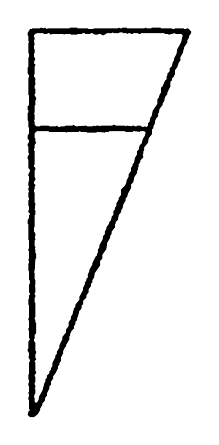
\begin{tikzpicture}[x=0.00979592cm,y=-0.00979592cm]
\fill[even odd rule] (224,12) -- (222,12) -- (221,13) -- (219,13) -- (218,12) -- (207,12) -- (206,13) -- (204,13) -- (203,12) -- (189,12) -- (188,11) -- (177,11) -- (176,12) -- (170,12) -- (169,11) -- (167,12) -- (145,12) -- (144,11) -- (139,11) -- (138,12) -- (136,12) -- (134,11) -- (133,12) -- (102,12) -- (101,13) -- (95,13) -- (94,12) -- (81,12) -- (80,11) -- (71,11) -- (70,12) -- (42,12) -- (41,13) -- (38,11) -- (37,12) -- (33,11) -- (32,12) -- (22,12) -- (21,13) -- (19,13) -- (16,18) -- (16,21) -- (17,22) -- (17,28) -- (18,29) -- (17,31) -- (17,44) -- (18,45) -- (18,49) -- (17,50) -- (17,62) -- (16,63) -- (16,70) -- (18,73) -- (18,75) -- (17,76) -- (17,98) -- (18,99) -- (18,111) -- (16,113) -- (16,117) -- (17,118) -- (17,121) -- (16,122) -- (16,131) -- (17,132) -- (17,140) -- (18,141) -- (18,148) -- (16,151) -- (16,155) -- (18,157) -- (18,159) -- (16,162) -- (16,164) -- (17,165) -- (17,173) -- (18,175) -- (16,178) -- (16,181) -- (17,182) -- (17,193) -- (19,195) -- (19,197) -- (17,201) -- (17,203) -- (18,204) -- (18,210) -- (17,211) -- (17,216) -- (18,217) -- (17,219) -- (17,222) -- (18,223) -- (17,225) -- (17,231) -- (18,232) -- (18,234) -- (17,235) -- (17,242) -- (18,243) -- (18,247) -- (17,248) -- (17,250) -- (19,252) -- (19,253) -- (18,254) -- (18,257) -- (16,261) -- (16,265) -- (17,266) -- (17,286) -- (18,287) -- (18,297) -- (17,298) -- (17,300) -- (18,301) -- (18,310) -- (17,311) -- (18,316) -- (17,317) -- (17,326) -- (18,327) -- (18,338) -- (19,339) -- (19,343) -- (18,344) -- (18,354) -- (19,355) -- (19,357) -- (18,358) -- (18,362) -- (17,363) -- (17,370) -- (18,371) -- (18,387) -- (17,388) -- (17,390) -- (18,391) -- (18,400) -- (17,401) -- (17,403) -- (18,404) -- (18,413) -- (19,415) -- (17,418) -- (17,427) -- (16,428) -- (16,430) -- (18,433) -- (18,436) -- (17,438) -- (19,442) -- (19,444) -- (18,445) -- (18,460) -- (17,461) -- (17,467) -- (18,468) -- (18,471) -- (17,472) -- (17,475) -- (18,476) -- (18,483) -- (17,484) -- (18,489) -- (17,490) -- (17,493) -- (18,494) -- (18,505) -- (19,507) -- (17,509) -- (16,513) -- (19,516) -- (24,516) -- (29,512) -- (32,507) -- (32,505) -- (35,500) -- (35,498) -- (38,495) -- (39,490) -- (41,488) -- (41,485) -- (44,479) -- (44,476) -- (46,474) -- (46,470) -- (49,466) -- (49,463) -- (52,459) -- (55,453) -- (55,450) -- (57,448) -- (57,446) -- (59,443) -- (59,439) -- (62,433) -- (62,430) -- (64,426) -- (66,424) -- (66,422) -- (70,415) -- (70,411) -- (71,410) -- (71,408) -- (73,404) -- (76,401) -- (76,398) -- (78,395) -- (78,392) -- (80,390) -- (80,387) -- (81,386) -- (83,378) -- (85,376) -- (86,374) -- (86,371) -- (88,369) -- (88,365) -- (92,361) -- (92,358) -- (95,354) -- (95,350) -- (98,346) -- (98,343) -- (100,341) -- (100,338) -- (102,335) -- (103,329) -- (110,319) -- (110,313) -- (113,310) -- (113,305) -- (118,298) -- (119,290) -- (123,283) -- (123,281) -- (125,278) -- (125,275) -- (129,270) -- (129,266) -- (130,265) -- (130,263) -- (133,260) -- (134,254) -- (137,250) -- (137,248) -- (139,245) -- (140,240) -- (143,235) -- (143,232) -- (145,230) -- (146,226) -- (150,219) -- (150,214) -- (153,211) -- (154,205) -- (158,199) -- (158,196) -- (159,195) -- (159,192) -- (160,191) -- (160,188) -- (162,185) -- (162,183) -- (166,179) -- (165,175) -- (166,174) -- (166,171) -- (167,170) -- (167,166) -- (172,160) -- (173,154) -- (177,149) -- (177,143) -- (179,141) -- (179,139) -- (181,135) -- (181,132) -- (183,128) -- (185,126) -- (185,122) -- (186,121) -- (187,116) -- (191,111) -- (191,109) -- (193,106) -- (194,101) -- (197,97) -- (197,95) -- (201,87) -- (201,81) -- (203,79) -- (203,77) -- (205,75) -- (207,71) -- (207,66) -- (210,62) -- (212,56) -- (214,54) -- (214,49) -- (217,44) -- (219,36) -- (223,30) -- (223,27) -- (225,24) -- (225,22) -- (228,18) -- (228,16) -- cycle
(167,145) -- (169,147) -- (168,151) -- (165,156) -- (164,161) -- (161,164) -- (160,169) -- (158,171) -- (158,175) -- (155,180) -- (154,186) -- (152,188) -- (152,190) -- (150,193) -- (150,197) -- (147,201) -- (147,204) -- (144,210) -- (144,212) -- (142,216) -- (137,221) -- (137,228) -- (134,232) -- (134,234) -- (131,239) -- (131,242) -- (129,245) -- (129,247) -- (127,249) -- (127,254) -- (125,256) -- (124,261) -- (122,263) -- (121,266) -- (118,270) -- (118,272) -- (116,276) -- (116,279) -- (114,281) -- (113,286) -- (109,293) -- (109,296) -- (107,299) -- (107,303) -- (106,304) -- (106,306) -- (104,308) -- (100,316) -- (100,318) -- (96,325) -- (96,327) -- (94,331) -- (94,335) -- (92,337) -- (92,339) -- (90,342) -- (90,344) -- (88,348) -- (88,351) -- (83,360) -- (83,364) -- (78,370) -- (78,373) -- (76,375) -- (74,383) -- (72,386) -- (72,389) -- (69,393) -- (69,398) -- (66,402) -- (66,406) -- (61,412) -- (61,415) -- (57,423) -- (57,426) -- (54,431) -- (54,434) -- (52,436) -- (52,438) -- (48,446) -- (48,450) -- (46,453) -- (46,455) -- (44,457) -- (44,459) -- (41,462) -- (41,465) -- (39,467) -- (39,470) -- (38,471) -- (35,482) -- (31,489) -- (30,494) -- (28,497) -- (26,497) -- (25,496) -- (25,491) -- (24,490) -- (25,486) -- (26,485) -- (26,480) -- (25,479) -- (26,477) -- (26,475) -- (25,474) -- (25,471) -- (26,470) -- (26,464) -- (25,463) -- (25,461) -- (27,459) -- (27,457) -- (26,456) -- (26,445) -- (25,444) -- (25,443) -- (27,441) -- (26,439) -- (26,434) -- (27,433) -- (27,431) -- (26,430) -- (26,420) -- (24,417) -- (24,415) -- (25,414) -- (25,409) -- (27,407) -- (27,394) -- (26,393) -- (26,390) -- (25,389) -- (25,387) -- (26,386) -- (26,368) -- (25,367) -- (25,361) -- (26,360) -- (26,358) -- (25,357) -- (25,355) -- (26,354) -- (26,348) -- (25,347) -- (26,346) -- (25,345) -- (26,344) -- (26,338) -- (25,337) -- (25,329) -- (24,328) -- (25,326) -- (26,311) -- (27,310) -- (27,304) -- (26,303) -- (26,299) -- (25,298) -- (26,296) -- (25,294) -- (25,287) -- (26,286) -- (25,282) -- (26,281) -- (26,278) -- (24,275) -- (24,270) -- (25,269) -- (25,254) -- (26,253) -- (26,248) -- (25,247) -- (26,239) -- (25,238) -- (25,225) -- (24,224) -- (24,221) -- (25,220) -- (25,217) -- (26,216) -- (26,215) -- (24,213) -- (24,211) -- (26,208) -- (26,206) -- (25,205) -- (25,196) -- (26,195) -- (26,193) -- (24,191) -- (24,189) -- (25,188) -- (25,171) -- (24,170) -- (24,168) -- (25,167) -- (25,163) -- (27,160) -- (26,159) -- (26,155) -- (25,154) -- (25,148) -- (28,145) -- (43,145) -- (44,146) -- (65,146) -- (66,147) -- (68,146) -- (82,146) -- (83,145) -- (85,146) -- (92,146) -- (93,147) -- (105,147) -- (106,146) -- (116,147) -- (117,146) -- (121,146) -- (122,145) -- (142,145) -- (143,146) -- (152,146) -- (153,145) -- (161,146) -- (162,145) -- cycle
(217,21) -- (215,30) -- (210,39) -- (209,45) -- (206,51) -- (206,53) -- (204,56) -- (203,61) -- (200,64) -- (200,68) -- (197,71) -- (197,73) -- (196,74) -- (196,78) -- (194,80) -- (191,87) -- (189,89) -- (189,95) -- (187,98) -- (186,102) -- (184,104) -- (184,110) -- (178,119) -- (177,125) -- (175,128) -- (174,133) -- (172,135) -- (172,138) -- (170,140) -- (168,139) -- (165,140) -- (162,138) -- (158,138) -- (157,139) -- (155,139) -- (154,138) -- (152,138) -- (151,139) -- (145,138) -- (143,139) -- (142,138) -- (130,138) -- (129,137) -- (127,137) -- (126,138) -- (111,138) -- (110,139) -- (108,138) -- (105,138) -- (104,139) -- (102,138) -- (100,139) -- (93,139) -- (92,138) -- (79,139) -- (75,137) -- (74,138) -- (65,138) -- (64,139) -- (59,139) -- (58,140) -- (56,140) -- (54,138) -- (52,139) -- (44,139) -- (43,138) -- (33,138) -- (32,139) -- (27,139) -- (25,137) -- (25,133) -- (24,132) -- (25,130) -- (25,124) -- (24,122) -- (25,121) -- (25,112) -- (26,111) -- (26,105) -- (27,104) -- (27,102) -- (25,99) -- (25,97) -- (26,96) -- (26,91) -- (25,90) -- (25,86) -- (26,85) -- (26,82) -- (25,80) -- (26,79) -- (26,77) -- (24,74) -- (24,72) -- (25,71) -- (25,61) -- (26,60) -- (26,59) -- (24,57) -- (25,53) -- (26,52) -- (24,48) -- (24,45) -- (25,44) -- (25,39) -- (24,38) -- (24,34) -- (25,33) -- (24,27) -- (25,26) -- (25,24) -- (24,23) -- (24,21) -- (26,19) -- (28,18) -- (36,18) -- (37,19) -- (41,19) -- (42,18) -- (44,18) -- (46,20) -- (48,19) -- (62,19) -- (63,20) -- (65,19) -- (71,19) -- (72,20) -- (80,20) -- (81,19) -- (86,19) -- (87,18) -- (90,18) -- (91,19) -- (97,19) -- (98,18) -- (100,18) -- (103,20) -- (107,20) -- (108,19) -- (110,19) -- (114,21) -- (119,18) -- (125,18) -- (126,17) -- (128,18) -- (134,18) -- (135,17) -- (139,17) -- (140,18) -- (144,18) -- (145,19) -- (147,18) -- (149,18) -- (150,19) -- (152,19) -- (153,18) -- (159,18) -- (160,19) -- (162,19) -- (163,18) -- (193,18) -- (194,19) -- (198,19) -- (199,20) -- (207,18) -- (208,19) -- (215,19) -- cycle;
\end{tikzpicture}
\end{center}

\[
dfx = fdx\,.\,gx.
\]

\noindent Es sei

\[
fdx = \alpha dx, \qquad fx = y;
\]

\noindent so ist

\[
\frac{dy}{dx} = \alpha gx,
\]
